%==============================================================================
%  CISC-727 — Assignment A05: ARE-II Ready Package
%  Author: Kenneth Peter Fernandes
%  Harrisburg University of Science and Technology
%  Instructor: Professor Majid Shaalan, Ph.D.
%==============================================================================
\documentclass[11pt]{article}

\usepackage[margin=1in]{geometry}
\usepackage[T1]{fontenc}
\usepackage[utf8]{inputenc}
\usepackage{mathptmx}
\usepackage{setspace}
\usepackage{parskip}
\usepackage{titlesec}
\usepackage{enumitem}
\usepackage{hyperref}
\usepackage{graphicx}
\usepackage{booktabs}
\usepackage{xcolor}
\usepackage{csquotes}
\usepackage{tabularx}
\usepackage{longtable}
\usepackage{array}
\usepackage{tikz}
\usetikzlibrary{trees, positioning, shapes.geometric, arrows.meta}

\usepackage[style=apa,backend=biber,sortcites=true]{biblatex}
\DeclareLanguageMapping{american}{american-apa}
\addbibresource{references.bib}

\hypersetup{
    colorlinks=true,
    linkcolor=blue,
    citecolor=blue,
    urlcolor=blue,
}

\onehalfspacing

\titleformat{\section}{\normalfont\large\bfseries}{\thesection.}{0.5em}{}
\titleformat{\subsection}{\normalfont\normalsize\bfseries}{\thesubsection.}{0.5em}{}
\titleformat{\subsubsection}{\normalfont\normalsize\bfseries\itshape}{\thesubsubsection.}{0.5em}{}

\title{%
    \vspace{0.5in}
    \textbf{ARE-II Ready Package}\\[0.3em]
    \large Proposal Skeleton, Method and Evaluation Protocol, Pilot Evidence,\\
    Related Work Map, and ARE-II Execution Plan\\[1em]
    \large CISC-727 --- Advanced Research Explorations (ARE) - I\\[0.2em]
    \large Assignment A05\\[1em]
}
\author{%
    Kenneth Peter Fernandes\\
    Department of Computer and Information Sciences\\
    Harrisburg University of Science and Technology\\[0.5em]
    Instructor: Prof.\ Majid Shaalan, Ph.D.
}
\date{April 25, 2026}

\begin{document}

\maketitle
\thispagestyle{empty}
\newpage

\tableofcontents
\newpage

%==============================================================================
\section*{Abstract}
\addcontentsline{toc}{section}{Abstract}
%==============================================================================

This package consolidates the work of CISC-727 (ARE-I) into a single, advisor-ready research bundle and proposes the next-semester (CISC-733, ARE-II) execution plan. The semester opened with a research interest in making long-context Large Language Model inference cheaper through IO-aware attention kernels and Key-Value cache management on commodity GPUs. The literature review (A02) narrowed this to a controlled question that is feasible on a single GPU: \textit{at what sequence-length and hardware conditions does an exact IO-aware attention kernel deliver meaningful efficiency gains over standard attention?} The pilot work (A03 and A04) used a Vision Transformer on CIFAR-10 and a Tesla T4 (Turing-class) GPU on Kaggle, sweeping partition granularity to vary sequence length from 5 to 65 tokens. The pilot reported a null-to-negative result: FlashAttention showed near-zero speedup at 5 tokens and was approximately sixteen percent slower than standard attention at 65 tokens. Late-stage investigation, captured in this package, revealed an important confound: PyTorch's \texttt{SDPBackend.FLASH\_ATTENTION} path requires Streaming Multiprocessor capability 8.0 or newer (Ampere or newer), and the Tesla T4 is Streaming Multiprocessor capability 7.5 (Turing). The pilot likely measured a silent fallback to a different attention implementation rather than the FlashAttention kernel itself. Because the population of researchers using the Tesla T4 through Kaggle and the free tier of Google Colab is large, this confound is itself worth measuring rigorously. ARE-II is therefore proposed as a four-sprint plan: (1) kernel attribution on Tesla T4 using profiler traces and warning logs, (2) a controlled microbenchmark sweep across sequence lengths from 64 to 4{,}096 tokens, (3) full-model validation that the microbenchmark crossover holds end-to-end, and (4) an optional Ampere-class spot check on a NVIDIA A100 to compare crossover regimes across GPU classes. The reproducible repository associated with this package contains the configurations, scripts, and pilot outputs needed for an advisor to reproduce the primary figure and to begin the ARE-II execution plan with minimal rework.

\newpage

%==============================================================================
\part*{Part I --- Proposal Skeleton}
\addcontentsline{toc}{part}{Part I --- Proposal Skeleton}
%==============================================================================

\section{Problem Statement}

Transformer-based models dominate modern machine learning workloads, yet the canonical scaled dot-product attention they rely on has cost that grows quadratically with sequence length~\parencite{vaswani2023attentionneed}. As context windows grow, the cost of attention dominates wall-clock time and memory footprint, especially on memory-bandwidth-limited GPUs. The community has responded with three broad families of remedies: (1) IO-aware exact attention kernels that preserve the attention math but rearrange memory traffic, exemplified by FlashAttention~\parencite{dao2022flashattentionfastmemoryefficientexact, dao2023flashattention2fasterattentionbetter, shah2024flashattention3fastaccurateattention}; (2) sparse attention that constrains the connectivity pattern~\parencite{beltagy2020longformerlongdocumenttransformer, zaheer2021bigbirdtransformerslonger}; and (3) linear or low-rank approximations of the attention operator~\parencite{wang2020linformerselfattentionlinearcomplexity, choromanski2022rethinkingattentionperformers, xiong2021nystromformernystrombasedalgorithmapproximating}. Although the FlashAttention family has become a de facto deployment default for newer GPUs, the published evidence base for FlashAttention is concentrated on data-center class accelerators (NVIDIA A100 and H100) and on training-time microbenchmarks. The behavior of attention kernels on Turing-class GPUs (NVIDIA Tesla T4 and the GeForce RTX 2080 family) has not been systematically characterized. This matters because the Tesla T4 is the most widely available free-tier accelerator for graduate research and for educational use. Free-tier offerings on Kaggle and on Google Colab provision the Tesla T4 by default, and a substantial population of compute-constrained researchers depends on this hardware. Two specific hazards arise on the Tesla T4: PyTorch's \texttt{torch.nn.functional.scaled\_dot\_product\_attention} dispatcher silently falls back to a non-FlashAttention path because the FlashAttention SDPA backend requires Streaming Multiprocessor capability 8.0 or newer~\parencite{pytorch2024sdpa}, and the official \texttt{flash-attn} package from Dao-AILab does not provide a stable installation for the Tesla T4 sm\_75 architecture~\parencite{flashattn_t4_issue887}. The combination produces a measurable but undocumented regime: researchers running attention experiments on the Tesla T4 may believe they are exercising FlashAttention while in fact exercising the standard math kernel or the memory-efficient kernel. The present work proposes to measure exactly that regime.

\section{Research Gap and Novelty Paragraph}

The literature has converged on FlashAttention v1, v2, and v3 as the canonical IO-aware attention implementation, and on the PagedAttention serving stack as the canonical Key-Value cache memory manager~\parencite{kwon2023efficientmemorymanagementlarge}. Surveys situate these as adjacent but distinct optimizations of the standard attention operator~\parencite{10.1145/3530811, sun2026efficientattentionmechanismslarge}. Benchmarks such as Long Range Arena~\parencite{tay2020longrangearenabenchmark} and the Comprehensive Attention Benchmark~\parencite{zhang2025cabcomprehensiveattentionbenchmarking} catalogue the relative quality of these methods across attention patterns and sequence lengths, and the Comprehensive Attention Benchmark introduces the useful concept of an \textit{efficiency length} above which an efficient method first surpasses standard attention. A 2025 contribution~\parencite{bu2025longcontextattentionbenchmark} extends kernel-level evaluation to distributed context parallelism on clusters of up to ninety-six accelerators. None of these resources, however, addresses the single-GPU, Turing-class regime that defines the realistic compute envelope for non-funded graduate research. The gap, stated precisely, is that the community lacks a controlled, reproducible characterization of (a) which attention kernel actually executes on the Tesla T4 under common API calls, (b) how the available kernels compare across sequence length and precision on the Tesla T4, and (c) the practical implications of that comparison for researchers who use Kaggle and free-tier Google Colab as their primary compute. This package proposes to close that gap. The novelty is not a new attention algorithm or kernel. The novelty is a controlled, single-GPU, Turing-class measurement study that reports kernel attribution, a sequence-length crossover map, and reproducible artifacts for the most-used free-tier accelerator in the field. The closest competitor publications report on Ampere or Hopper accelerators only, evaluate only kernels that are unsupported on the Tesla T4, or report on multi-accelerator distributed evaluation~\parencite{dao2022flashattentionfastmemoryefficientexact, dao2023flashattention2fasterattentionbetter, bu2025longcontextattentionbenchmark}.

\section{Research Questions and Hypotheses}

\subsection{Primary research question}
On a Tesla T4 (Streaming Multiprocessor capability 7.5, Turing-class), under common PyTorch API calls and for sequence lengths in the range 64 to 4{,}096 tokens, which attention kernel actually executes, and at what sequence length does the memory-efficient implementation surpass the standard math implementation in wall-clock time per call and in peak memory?

\subsection{Falsifiable hypotheses}
\begin{description}[leftmargin=2em]
    \item[Hypothesis~1 (kernel attribution).] When PyTorch is asked for the FlashAttention SDPA backend on a Tesla T4 in 2026, the dispatched CUDA kernel will not match a FlashAttention v1, v2, or v3 kernel. \textit{Refutation condition:} a profiler trace that shows a Dao-AILab FlashAttention CUDA kernel name in the rank-zero call stack on a Tesla T4.
    \item[Hypothesis~2 (crossover existence).] At sequence lengths beyond 512 tokens on a Tesla T4 with FP16 precision, the PyTorch memory-efficient SDPA backend will deliver lower median wall-clock time per call than the standard math backend by at least ten percent. \textit{Refutation condition:} no crossover up to 4{,}096 tokens, or a crossover that falls below the ten-percent margin under matched conditions.
    \item[Hypothesis~3 (kernel parity).] At long sequences (1{,}024 tokens and above) on a Tesla T4 with FP16 precision, the xFormers \texttt{memory\_efficient\_attention} operator will achieve median wall-clock time within ten percent of PyTorch's memory-efficient SDPA backend. \textit{Refutation condition:} a sustained gap above ten percent in either direction.
\end{description}
These three hypotheses are internally consistent. Hypothesis~1 establishes what is being measured. Hypothesis~2 establishes whether anything is to be gained from the kernel-aware choice on the Tesla T4. Hypothesis~3 establishes whether xFormers and PyTorch SDPA are interchangeable for this regime, which has practical importance for compute-constrained researchers who must depend on whichever installs cleanly.

\section{Proposed Contributions}
\begin{enumerate}[leftmargin=2em]
    \item \textbf{A kernel-attribution methodology for the Tesla T4} that combines PyTorch's SDPA dispatcher API, the PyTorch profiler, and PyTorch's warning log to record, per attention call, the actual CUDA kernel signature that executes. This is implemented in code as a small wrapper utility plus a YAML-driven configuration sweep.
    \item \textbf{A crossover map for the attention kernels available on a Tesla T4} (math, memory-efficient SDPA, xFormers memory-efficient), reported across sequence lengths 64 to 4{,}096 tokens and across FP16 and FP32 precisions, with median and inter-quartile range.
    \item \textbf{Full-model validation} that the microbenchmark crossover holds in an end-to-end training step on a Vision Transformer at sequence lengths consistent with the microbenchmark axis.
    \item \textbf{A reproducible repository} that an advisor can clone and run on Kaggle to reproduce the primary figure with a single command, including the cleaned harness used in the A03 and A04 pilot, the ARE-II configurations, and the pilot logs.
\end{enumerate}

\section{Method Overview}

The high-level approach is empirical: a controlled sweep over the independent variables (sequence length, kernel selection, and precision) on a single Tesla T4, with median wall-clock time per call and peak GPU memory as the dependent variables. Every measurement is preceded by a kernel-attribution check that records which kernel was actually launched. The microbenchmark uses a single attention layer with embedding dimension 384 and six heads (matched to the A03 and A04 Vision Transformer harness), batch size 16, ten warmup iterations, and fifty measured iterations per cell. Three repetitions per cell support nonparametric reporting (median and inter-quartile range). Kernel attribution is performed via the PyTorch profiler and through capturing PyTorch's warning emissions on backend selection failure. Full-model validation reuses the A03 and A04 distributed training harness with sequence length increased by upscaling the input image and reducing the patch size. No new attention algorithm is introduced. The work is methodologically aligned with the partitioning, communication, agglomeration, and mapping framing common in parallel-computing research: the partition is a single attention call, the communication is reduced to host-device synchronization for timing, the agglomeration is the choice of batch size and sequence length, and the mapping is the kernel selection.

\section{Evaluation Plan Summary}

The evaluation reports five quantities per (kernel, precision, sequence length) cell. First, the kernel signature actually launched, recorded by the profiler. Second, the median wall-clock time per call, in milliseconds, with inter-quartile range over three repetitions of fifty measured iterations. Third, the peak GPU memory in megabytes, recorded from \texttt{torch.cuda.max\_memory\_allocated}. Fourth, an indicator of whether the requested kernel matched the launched kernel (a boolean derived from the kernel signature). Fifth, the PyTorch warning text emitted, if any, on backend selection. Three baselines are reported: PyTorch \texttt{SDPBackend.MATH} (standard attention), PyTorch \texttt{SDPBackend.EFFICIENT\_ATTENTION} (memory-efficient), and PyTorch \texttt{SDPBackend.FLASH\_ATTENTION} (which is expected to fall back on Tesla T4). One literature-aligned alternative kernel is reported: xFormers \texttt{memory\_efficient\_attention}~\parencite{xformers2022}. Pre-registered ablations vary precision (FP16, FP32) and sequence length on the same axes. Success for ARE-II is defined as: a kernel-attribution table for all reported runs, a crossover plot with at least two kernels showing a clear crossover at or below 4{,}096 tokens, and a successful end-to-end full-model run at sequence length 1{,}025 or higher. The four metrics together support the falsifiability statement of each hypothesis.

\section{Risks and Mitigations}

The principal technical risks are summarized in Table~\ref{tab:risks-summary}. The risk register is fuller in Part~III (Method and Evaluation Protocol).

\begin{table}[h!]
\centering
\caption{Top-five technical risks with mitigations}
\label{tab:risks-summary}
\small
\begin{tabularx}{\textwidth}{p{4.2cm} X}
\toprule
\textbf{Risk} & \textbf{Mitigation and fallback} \\
\midrule
Free-tier Tesla T4 weekly compute quota (Kaggle: approximately 30 GPU-hours per week) limits sweep size & Stagger sweep across two weekends; checkpoint between sessions; reduce repetitions to 2 if necessary. \\
Kernel attribution surfaces unexpected behavior (for example, the dispatcher routes \texttt{FLASH\_ATTENTION} to memory-efficient on Tesla T4) & This is a useful negative result and is reported as such. The hypothesis structure already anticipates this outcome. \\
\texttt{flash-attn} v1.x will not install reliably on Tesla T4 in 2026~\parencite{flashattn_t4_issue887} & The \texttt{flash-attn} pip package is excluded from the Tesla T4 path. xFormers is the substitute. The Ampere spot check (Sprint~4) uses real FlashAttention. \\
Tesla T4 is deprecated or replaced on Kaggle and Colab during the ARE-II window & Re-run on the replacement free-tier accelerator and report behavior on the replacement; the methodology is portable. \\
Time budget loss to a missed weekend & Stretch goal (Sprint~4) is dropped first; full-model validation (Sprint~3) is reduced to two sequence lengths; writing weekends are protected. \\
\bottomrule
\end{tabularx}
\end{table}

\section{ARE-II Execution Plan}
\label{sec:areii-plan}

The ARE-II window is May~9 through the first week of August, with weekend-only working hours and use of AI tools for boilerplate and writing assistance only. The plan budgets approximately eleven productive weekends, reserves two to three for writing the final committee report and figure polishing, and treats the Ampere spot check as a stretch goal. The four sprints are summarized in Table~\ref{tab:areii-sprints}; the calendar appears in Table~\ref{tab:areii-calendar}.

\begin{table}[h!]
\centering
\caption{ARE-II sprints, deliverables, and weekend budget}
\label{tab:areii-sprints}
\small
\begin{tabularx}{\textwidth}{l X p{2.8cm}}
\toprule
\textbf{Sprint} & \textbf{Deliverable} & \textbf{Weekend budget} \\
\midrule
1. Kernel attribution & Kernel signatures and warning logs per backend on Tesla T4; verification table for the three SDPA backends and xFormers; resolution of the A04 ambiguity. & 1 weekend \\
2. Microbenchmark & Crossover map of time per call and peak memory across three kernels, two precisions, and seven sequence lengths on Tesla T4. The headline ARE-II figure. & 3 weekends \\
3. Full-model validation & End-to-end ViT runs at increased sequence length (up to approximately 3{,}137 tokens) showing whether the microbenchmark crossover holds in training. & 2 to 3 weekends \\
4. A100 spot check (stretch) & Re-run of the Sprint~2 sweep on an Ampere-class GPU (A100); cross-architecture comparison of crossover regimes; explicit verification that real FlashAttention v1 and v2 execute on Ampere. & 1 weekend (drop if Sprint~3 is late) \\
\midrule
Writing and polish & Committee report, figures, reproducibility cleanup. & 2 to 3 weekends \\
\bottomrule
\end{tabularx}
\end{table}

\begin{table}[h!]
\centering
\caption{ARE-II weekend calendar (May 9 to August first week, 2026)}
\label{tab:areii-calendar}
\small
\begin{tabularx}{\textwidth}{l l X}
\toprule
\textbf{Index} & \textbf{Weekend} & \textbf{Plan} \\
\midrule
W1 & May 10--11 & Sprint 1: environment setup, profiler harness, kernel attribution. \\
W2 & May 17--18 & Sprint 2 setup and first sweep run. \\
-- & May 24--26 & Memorial Day weekend; skipped. \\
W4 & May 31--Jun 1 & Sprint 2: full sweep and analysis. \\
W5 & Jun 7--8 & Sprint 2: ablations and fixes. \\
W6 & Jun 14--15 & Sprint 3: full-model harness extension. \\
W7 & Jun 21--22 & Sprint 3: full-model runs. \\
W8 & Jun 28--29 & Sprint 3: analysis and buffer. \\
-- & Jul 4--6 & July 4 weekend; skipped. \\
W10 & Jul 12--13 & Buffer or Sprint 4 stretch (only if on track). \\
W11 & Jul 19--20 & Writing: figures and committee report draft. \\
W12 & Jul 26--27 & Writing: revision. \\
W13 & Aug 2--3 & Final polish and submission. \\
\bottomrule
\end{tabularx}
\end{table}

\noindent The plan has one hard checkpoint: by July 5, if Sprint~3 is not complete, Sprint~4 is dropped without remorse and the writing weekends are protected. The hardware path prioritizes (in order) Harrisburg University internal high-performance computing, an AWS Cloud Credit for Research grant if approved, RunPod Secure Cloud at approximately one US dollar twenty-nine cents per A100 hour for a budget of approximately thirty US dollars, and otherwise drops the Sprint~4 stretch goal. The IP profile of the work is preserved: free Kaggle and free Colab are governed by their respective terms (acceptable for unpublished pre-publication work), and the candidate paid platform is RunPod Secure Cloud which retains user IP explicitly in its terms of service. Lambda Labs is excluded from the candidate pool because of broad license clauses in its terms of service, and Vast.ai's hobbyist tier is excluded because of unverified host machines.

\newpage

%==============================================================================
\part*{Part II --- Related Work Package}
\addcontentsline{toc}{part}{Part II --- Related Work Package}
%==============================================================================

\section{Literature Map}
\label{sec:lit-map}

The literature relevant to this work falls into six clusters: (1) the foundational Transformer baseline; (2) survey and taxonomy literature; (3) IO-aware exact attention (FlashAttention family); (4) Key-Value cache management and head-sharing for inference; (5) sparse and linear/low-rank approximate attention; and (6) benchmark and evaluation frameworks. Figure~\ref{fig:lit-map} shows the visual taxonomy in tree form. Each cluster is summarized in Section~\ref{sec:annotated-bib}, where every cited work appears in the annotated bibliography table.

\begin{figure}[h!]
\centering
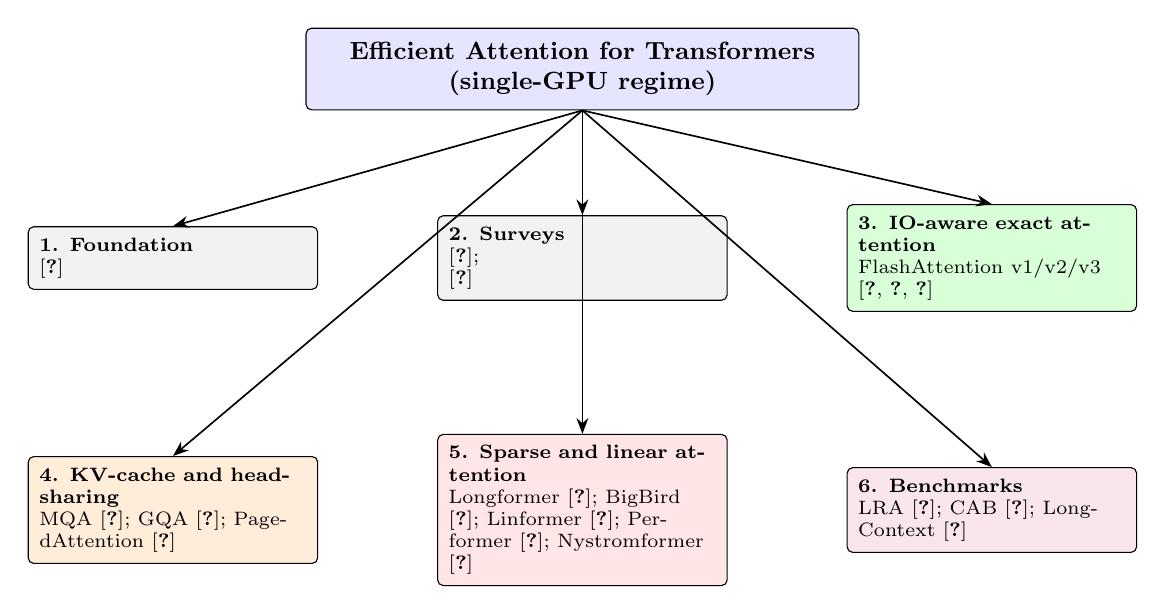
\begin{tikzpicture}[
    every node/.style={font=\scriptsize, align=left},
    box/.style={rectangle, draw, rounded corners=2pt, text width=0.28\textwidth, inner sep=4pt},
    rootbox/.style={rectangle, draw, rounded corners=2pt, fill=blue!10, text width=0.55\textwidth, align=center, inner sep=5pt, font=\small\bfseries},
]
% Root
\node[rootbox] (root) at (0,0) {Efficient Attention for Transformers\\(single-GPU regime)};

% Row 1 (clusters 1, 2, 3)
\node[box, fill=gray!10] (foundation) at (-5.2, -2.4)
  {\textbf{1. Foundation}\\
   \cite{vaswani2023attentionneed}};
\node[box, fill=gray!10] (survey) at (0, -2.4)
  {\textbf{2. Surveys}\\
   \cite{10.1145/3530811};\\
   \cite{sun2026efficientattentionmechanismslarge}};
\node[box, fill=green!15] (ioaware) at (5.2, -2.4)
  {\textbf{3. IO-aware exact attention}\\
   FlashAttention v1/v2/v3
   \cite{dao2022flashattentionfastmemoryefficientexact, dao2023flashattention2fasterattentionbetter, shah2024flashattention3fastaccurateattention}};

% Row 2 (clusters 4, 5, 6)
\node[box, fill=orange!15] (kv) at (-5.2, -5.6)
  {\textbf{4. KV-cache and head-sharing}\\
   MQA \cite{shazeer2019fasttransformerdecodingwritehead};
   GQA \cite{ainslie2023gqatraininggeneralizedmultiquery};
   PagedAttention \cite{kwon2023efficientmemorymanagementlarge}};
\node[box, fill=red!10] (sparse) at (0, -5.6)
  {\textbf{5. Sparse and linear attention}\\
   Longformer \cite{beltagy2020longformerlongdocumenttransformer};
   BigBird \cite{zaheer2021bigbirdtransformerslonger};
   Linformer \cite{wang2020linformerselfattentionlinearcomplexity};
   Performer \cite{choromanski2022rethinkingattentionperformers};
   Nystromformer \cite{xiong2021nystromformernystrombasedalgorithmapproximating}};
\node[box, fill=purple!10] (bench) at (5.2, -5.6)
  {\textbf{6. Benchmarks}\\
   LRA \cite{tay2020longrangearenabenchmark};
   CAB \cite{zhang2025cabcomprehensiveattentionbenchmarking};
   Long-Context \cite{bu2025longcontextattentionbenchmark}};

% Arrows from root to each cluster
\draw[->, >=Stealth, semithick] (root.south) -- (foundation.north);
\draw[->, >=Stealth, semithick] (root.south) -- (survey.north);
\draw[->, >=Stealth, semithick] (root.south) -- (ioaware.north);
\draw[->, >=Stealth, semithick] (root.south) -- (kv.north);
\draw[->, >=Stealth, semithick] (root.south) -- (sparse.north);
\draw[->, >=Stealth, semithick] (root.south) -- (bench.north);
\end{tikzpicture}
\caption{Literature taxonomy used for this work. The proposed contribution sits in the single-GPU intersection of Cluster~3 (IO-aware exact attention) and Cluster~6 (benchmarks).}
\label{fig:lit-map}
\end{figure}

\section{Gap Matrix}
\label{sec:gap-matrix}

Table~\ref{tab:gap-matrix} compares the closest competitors on the dimensions that matter for the proposed contribution: hardware regime evaluated, kernel actually exercised, sequence length range, whether kernel attribution is performed, whether the result is reproducible from the published artifacts, and whether the work covers the Tesla T4 specifically. The proposed contribution is the row labeled \textit{This work}.

\begin{table}[h!]
\centering
\caption{Gap matrix: closest-competitor comparison on six dimensions}
\label{tab:gap-matrix}
\footnotesize
\begin{tabularx}{\textwidth}{p{2.4cm} p{1.7cm} p{2.0cm} p{1.6cm} p{1.4cm} p{1.4cm} X}
\toprule
\textbf{Work} & \textbf{Hardware regime} & \textbf{Kernel exercised} & \textbf{Seq.\ length range} & \textbf{Kernel attribution?} & \textbf{Tesla T4 covered?} & \textbf{Distance from this work} \\
\midrule
FlashAttention v1 \cite{dao2022flashattentionfastmemoryefficientexact} & A100 & FlashAttention v1 & 128--64K & Implicit & No & Reports A100 only; no T4. \\
FlashAttention v2 \cite{dao2023flashattention2fasterattentionbetter} & A100 & FlashAttention v2 & 128--16K & Implicit & No & Requires sm\_80; not runnable on T4. \\
FlashAttention v3 \cite{shah2024flashattention3fastaccurateattention} & H100 & FlashAttention v3 & 1K--16K & Implicit & No & Hopper-specific; T4 not addressed. \\
PagedAttention/vLLM \cite{kwon2023efficientmemorymanagementlarge} & Multi-GPU server & Standard attention with paged KV & 1K--32K & No & No & Targets KV memory, not kernel choice. \\
Long Range Arena \cite{tay2020longrangearenabenchmark} & TPU/GPU (varied) & Multiple & 1K--16K & No & No & Quality benchmark; not kernel-level. \\
Comprehensive Attention Benchmark \cite{zhang2025cabcomprehensiveattentionbenchmarking} & GPU (varied) & Multiple & 1K--16K & No & Implicit only & Cross-pattern quality benchmark; no T4 kernel attribution. \\
Long-Context Attention Benchmark \cite{bu2025longcontextattentionbenchmark} & Cluster up to 96 GPUs & FlashAttention v2/v3 & 4K--256K & Yes & No & Multi-GPU; data-center class only. \\
\midrule
\textbf{This work} & \textbf{Tesla T4 (Turing, sm\_75)} & \textbf{Math, memory-efficient SDPA, xFormers; FlashAttention attempted} & \textbf{64--4{,}096} & \textbf{Yes (profiler-traced)} & \textbf{Yes} & --- \\
\bottomrule
\end{tabularx}
\end{table}

\section{Annotated Bibliography}
\label{sec:annotated-bib}

Eighteen sources are catalogued below with their relevance to the proposed contribution, the method type, the metrics they emphasize, their limitations, and notes on reproducibility. The set covers the foundation, the FlashAttention family, the Key-Value cache and head-sharing literature, sparse and linear approximate attention, benchmarks, surveys, and software references.

\begin{small}
\begin{longtable}{p{2.4cm} p{1.6cm} p{1.6cm} p{2.5cm} p{2.2cm} p{2.5cm}}
\caption{Annotated bibliography (18 sources)}
\label{tab:annot-bib} \\
\toprule
\textbf{Source} & \textbf{Method type} & \textbf{Metrics} & \textbf{Relevance to this work} & \textbf{Limitation} & \textbf{Reproducibility} \\
\midrule
\endfirsthead
\toprule
\textbf{Source} & \textbf{Method type} & \textbf{Metrics} & \textbf{Relevance to this work} & \textbf{Limitation} & \textbf{Reproducibility} \\
\midrule
\endhead
\bottomrule
\endfoot

\cite{vaswani2023attentionneed} & Foundation & BLEU, training cost & Defines the standard attention baseline. & No long-context evaluation. & Code released; reference implementations widely available. \\
\cite{10.1145/3530811} & Survey & Taxonomy & Provides the taxonomy used in Section~\ref{sec:lit-map}. & Not empirical. & Not applicable. \\
\cite{dao2022flashattentionfastmemoryefficientexact} & Exact, IO-aware & Time, memory, IO complexity & Anchor paper; defines the IO-aware framing. & Reports on A100 only. & Reference CUDA kernels released. \\
\cite{dao2023flashattention2fasterattentionbetter} & Exact, IO-aware & Time, FLOPs utilization & Improvement to v1; not runnable on T4. & Requires sm\_80 or newer. & Reference kernels released; T4 wheel unavailable. \\
\cite{shah2024flashattention3fastaccurateattention} & Exact, IO-aware & TFLOPs/s, FP8 numerics & Hopper-specific kernel; bounds the FlashAttention family. & H100-only. & Reference kernels released; H100 wheel only. \\
\cite{shazeer2019fasttransformerdecodingwritehead} & KV-cache reduction & Decoding speedup & Multi-Query Attention; orthogonal to the kernel-choice question. & Quality trade-offs reported only on small models. & Architecture is implementable from the paper. \\
\cite{ainslie2023gqatraininggeneralizedmultiquery} & KV-cache reduction & Throughput, quality & Grouped-Query Attention; widely deployed in modern LLMs. & Limited public reproductions on long context. & Architecture released; checkpoints not always public. \\
\cite{kwon2023efficientmemorymanagementlarge} & Serving system & Throughput, GPU memory & Closest serving-stack competitor in spirit. & Targets KV memory, not kernel selection. & vLLM open-source; Docker images available. \\
\cite{beltagy2020longformerlongdocumenttransformer} & Sparse attention & Task scores, runtime & Contrast family; not the focus of this work. & Implementation efficiency varies by task. & Code released. \\
\cite{zaheer2021bigbirdtransformerslonger} & Sparse attention & Task scores, theoretical expressivity & Contrast family. & Empirical and theoretical assumptions are coupled. & Code released. \\
\cite{wang2020linformerselfattentionlinearcomplexity} & Linear / low-rank & Time, memory, quality & Approximate attention contrast. & Low-rank assumption sensitive to task. & Code released. \\
\cite{choromanski2022rethinkingattentionperformers} & Linear / kernel-based & Time, memory, quality & Approximate attention contrast (FAVOR+). & Approximation quality varies. & Code released. \\
\cite{xiong2021nystromformernystrombasedalgorithmapproximating} & Linear / Nystr{\"o}m & Time, memory, quality & Approximate attention contrast. & Landmark-based approximation. & Code released. \\
\cite{tay2020longrangearenabenchmark} & Benchmark & Task scores & Established benchmark for long-range modeling. & Quality only; no kernel attribution. & Open. \\
\cite{zhang2025cabcomprehensiveattentionbenchmarking} & Benchmark & Cross-pattern quality, efficiency length & Introduces \textit{efficiency length}; methodologically aligned. & No T4 kernel-level reporting. & Open. \\
\cite{bu2025longcontextattentionbenchmark} & Benchmark & Kernel time, distributed throughput & Most recent kernel benchmark; multi-GPU only. & No single-T4 results. & Open. \\
\cite{sun2026efficientattentionmechanismslarge} & Survey & Taxonomy & Recent (2026) LLM-focused efficient-attention survey. & Not empirical. & Not applicable. \\
\cite{xformers2022} & Software & Time, memory & xFormers library; supports T4 (sm\_75) memory-efficient attention. & Documentation skews toward newer GPUs. & Open-source; pip-installable. \\
\end{longtable}
\end{small}

\section{Closest Competitor and How This Work Differs}

The closest competitor in spirit is the 2025 Long-Context Attention Benchmark~\parencite{bu2025longcontextattentionbenchmark}: it performs kernel-level attribution and characterizes time per call across kernels and configurations. It differs from this work along two essential axes. First, that work targets distributed clusters of up to ninety-six accelerators and reports on FlashAttention v2 and v3, which are not runnable on the Tesla T4. Second, that work does not consider Turing-class GPUs at all. The present work fills the single-GPU, Turing-class regime that the recent benchmark explicitly does not cover. The Comprehensive Attention Benchmark~\parencite{zhang2025cabcomprehensiveattentionbenchmarking} is closer in evaluation methodology (cross-pattern reporting; introduction of \textit{efficiency length}) but does not report kernel-attribution information at the granularity required for the present question. The novelty of the present work is therefore: a single-GPU Tesla T4 measurement study, with explicit kernel attribution, on the most-used free-tier accelerator for compute-constrained graduate research.

\newpage

%==============================================================================
\part*{Part III --- Method and Evaluation Protocol}
\addcontentsline{toc}{part}{Part III --- Method and Evaluation Protocol}
%==============================================================================

\section{System Under Test}

The system under test is a PyTorch-based attention measurement harness on a single NVIDIA Tesla T4 GPU. The Tesla T4 has 16 gigabytes of HBM2, Streaming Multiprocessor capability 7.5 (Turing architecture), peak FP16 throughput of approximately sixty-five TFLOPs (according to the device manufacturer), and uses PCIe interconnect when paired with another Tesla T4 (the multi-GPU configuration available on Kaggle). The software stack pins PyTorch at version 2.9 or newer, torchvision at 0.20 or newer, NumPy at 1.26 or newer, pandas at 2.2 or newer, and matplotlib at 3.8 or newer. The xFormers package, when used, is pinned at 0.0.28 or newer. The CUDA toolkit version is whatever Kaggle's runtime ships at the time of the experiment. The harness records the runtime environment in each run's output JSON: PyTorch version, CUDA version, xFormers version, kernel signature (when profiling is enabled), and GPU model.

\section{Workload, Model, and Data}

The microbenchmark workload is a single attention layer with embedding dimension 384 and six heads, batch size 16, sequence length swept across 64, 128, 256, 512, 1{,}024, 2{,}048, and 4{,}096 tokens (and 8{,}192 tokens conditional on memory headroom). The full-model workload is a Vision Transformer with the same embedding dimension and twelve transformer blocks, trained on CIFAR-10 with image upscaling and patch-size reduction to control sequence length (5, 65, 257, 1{,}025, and 3{,}137 tokens). The dataset is loaded from Kaggle's pre-mounted \texttt{cifar-10-python} input. No new dataset is collected.

\section{Partitioning, Communication, Agglomeration, and Mapping (PCAM)}

\begin{description}[leftmargin=2em]
    \item[Partitioning.] The unit of work is a single attention call. The microbenchmark partitions the work as one call per measurement iteration. The full-model run partitions across data-parallel replicas (DistributedDataParallel) when two Tesla T4 GPUs are available.
    \item[Communication.] The microbenchmark has no inter-process communication. The full-model run uses NCCL all-reduce for gradient synchronization. Communication is reported separately from compute via the forward-backward time decomposition that A04 used.
    \item[Agglomeration.] The agglomeration parameters are batch size 16 (microbenchmark) and 64 per GPU (full-model), held constant across kernels and precisions to support fair comparison.
    \item[Mapping.] Mapping is the kernel selection: math, memory-efficient SDPA, or xFormers. The mapping decision is the central independent variable of the study.
\end{description}

\section{Predicted Bottlenecks (Work-Depth Reasoning)}

Standard attention on a Tesla T4 with sequence length $n$ is expected to be HBM-bandwidth bound for $n$ in the low-thousand-token regime, because the materialization of the $n \times n$ score and weight matrices in HBM dominates. Memory-efficient attention is expected to be on-chip-bound (SRAM tile traffic) for the same regime, with a crossover where its lower HBM traffic outweighs its tile-management overhead. The crossover sequence length on a Tesla T4 is the central empirical question; the literature places the analogous crossover for FlashAttention on A100 in the 128 to 512 token range~\parencite{dao2022flashattentionfastmemoryefficientexact}, but the Tesla T4 has different HBM-to-SRAM bandwidth ratios and no native FlashAttention path, which is why the empirical map is required.

\section{Baselines}

Three baselines are reported. (1) PyTorch \texttt{SDPBackend.MATH} (standard attention) is the reference single-GPU baseline. (2) PyTorch \texttt{SDPBackend.EFFICIENT\_ATTENTION} (memory-efficient kernel) is the standard multi-GPU-class baseline that is literally available on Turing and forms the kernel-attribution endpoint that we expect the FlashAttention request to fall back to. (3) xFormers \texttt{memory\_efficient\_attention}~\parencite{xformers2022} is the literature-aligned alternative to PyTorch's memory-efficient SDPA path; it is included to verify whether the two implementations are interchangeable on Tesla T4. The PyTorch \texttt{SDPBackend.FLASH\_ATTENTION} request is logged separately as a \emph{kernel-attribution probe}, not as a fourth baseline, because its actual dispatched kernel on Tesla T4 is the open question.

\section{Metrics}

\begin{description}[leftmargin=2em]
    \item[Time per call (milliseconds).] Median of fifty measured iterations after ten warmup iterations, repeated three times. Inter-quartile range is reported alongside the median.
    \item[Peak GPU memory (megabytes).] \texttt{torch.cuda.max\_memory\_allocated} measured immediately after the call, then reset.
    \item[Kernel signature.] String name of the launched CUDA kernel as recorded by the PyTorch profiler. A single kernel signature per (kernel, precision, sequence length) cell is reported. Cells where the launched kernel does not match the requested kernel are flagged.
    \item[Backend warning text.] Any warning emitted by PyTorch when a backend is requested. The warning text is recorded verbatim.
    \item[Throughput proxy: tokens per second per GPU.] Derived from time per call and batch-times-sequence-length. Reported for full-model runs.
\end{description}

\section{Ablation Plan}

Ablations vary one factor at a time. (a) Precision is varied between FP16 and FP32 with kernel and sequence length held constant. (b) Sequence length is varied with kernel and precision held constant. (c) Kernel is varied with sequence length and precision held constant. (d) Batch size is held constant in the microbenchmark and varied in a small full-model ablation in Sprint~3.

\section{Measurement Protocol and Fairness Policy}

Each cell uses ten warmup iterations and fifty measured iterations. Repetitions per cell are three (for nonparametric reporting) for the microbenchmark and three for the full-model runs. The seed is fixed at 42 plus the local rank. CUDA event-based timing is used and host-device synchronization is performed before recording each event. Batch size is held constant across kernels for fairness. Mixed precision is exercised explicitly via the precision factor and is not interleaved.

\section{Threats to Validity}

\begin{description}[leftmargin=2em]
    \item[Construct validity (the most important threat in this work).] The PyTorch \texttt{SDPBackend.FLASH\_ATTENTION} request on a Tesla T4 may not execute the kernel implied by the name. The pilot evidence in Part~IV motivates this concern: the A03 and A04 results labelled \enquote{flash} may have measured a different kernel. The mitigation is the explicit kernel-attribution check in Sprint~1; until that check is performed, claims about FlashAttention behavior on Tesla T4 are stated cautiously, not assertively.
    \item[Internal validity.] Run-to-run variance from driver, scheduler, and thermal effects is bounded by the warmup-and-replicate protocol and reported via inter-quartile range rather than standard deviation.
    \item[External validity.] Conclusions are explicitly scoped to the Tesla T4 on Kaggle and Colab. Sprint~4 (the optional Ampere spot check) provides one cross-architecture data point; no claim is made about Hopper.
    \item[Reproducibility threat.] The Tesla T4 may be deprecated on free Kaggle and free Colab during the ARE-II window. The mitigation is the harness's portability: the harness will run on any Streaming Multiprocessor 7.5 or newer Tesla GPU with no code changes.
\end{description}

\section{Success Criteria}

ARE-II is considered to have produced evidence of contribution if all three of the following hold: (1) the kernel-attribution table for the three SDPA backends and xFormers is complete and reproducible from the repository; (2) the crossover plot shows a measurable crossover between at least two kernels at or below 4{,}096 tokens; and (3) the full-model run at sequence length 1{,}025 or higher executes successfully and is consistent with the microbenchmark crossover within the inter-quartile band. A null result on (2) is acceptable provided (1) is reported rigorously and (3) is replaced by a thorough mechanistic explanation.

\newpage

%==============================================================================
\part*{Part IV --- Pilot Evidence}
\addcontentsline{toc}{part}{Part IV --- Pilot Evidence}
%==============================================================================

\section{Baseline Reproduction Summary}

The A03 pilot reproduced single-GPU and multi-GPU baselines for a Vision Transformer on CIFAR-10, sweeping nine run identifiers (R1 through R9) covering single-GPU, DistributedDataParallel, and FullyShardedDataParallel parallelization strategies, with optional automatic mixed precision and explicit compute-communication overlap. The A03 baseline was validated against published distributed-training expectations: the median time per step on a single GPU (R1) was 0.035 seconds, and the multi-GPU runs (R3 through R9) showed scaling efficiency between approximately 0.27 and 0.30, consistent with the PCIe interconnect on Kaggle's two-Tesla T4 platform~\parencite{vaswani2023attentionneed}. The summary numbers from A03 are reproduced in Table~\ref{tab:a03-baseline}.

\begin{table}[h!]
\centering
\caption{A03 baseline reproduction summary (Vision Transformer on CIFAR-10, two Tesla T4)}
\label{tab:a03-baseline}
\small
\begin{tabularx}{\textwidth}{l X r r r}
\toprule
\textbf{Run} & \textbf{Strategy and kernel} & \textbf{Median time/step (s)} & \textbf{Throughput (samples/s)} & \textbf{Scaling eff.} \\
\midrule
R1 & Single GPU, math attention                 & 0.0350 & 1828.6 & 1.00 \\
R2 & Single GPU, FlashAttention (requested)     & 0.0359 & 1781.7 & 0.97 \\
R3 & DDP, math attention                        & 0.0598 & 2142.2 & 0.29 \\
R4 & DDP, FlashAttention (requested)            & 0.0591 & 2164.0 & 0.30 \\
R5 & FSDP, math attention                       & 0.0588 & 2175.3 & 0.30 \\
R6 & FSDP, FlashAttention (requested)           & 0.0589 & 2173.9 & 0.30 \\
R7 & DDP + FlashAttention + AMP                 & 0.0647 & 1978.9 & 0.27 \\
R8 & DDP + FlashAttention + Overlap             & 0.0591 & 2165.5 & 0.30 \\
R9 & DDP + FlashAttention + AMP + Overlap       & 0.0644 & 1987.7 & 0.27 \\
\bottomrule
\end{tabularx}
\end{table}

\section{Strong Result (Primary Figure)}

The A04 strong result varied a single lever from the A03 baseline: the partition granularity, implemented as the patch size in the Vision Transformer. A patch size of 16 produces 5 tokens per image; a patch size of 4 produces 65 tokens per image. The configuration is otherwise identical to the A03 R3/R4 baseline (two Tesla T4 GPUs on Kaggle, DistributedDataParallel, batch size 64 per GPU, 100 steps, 10 warmup, FP32, AdamW with learning rate 0.001, three repetitions per cell). The primary figure (Figure~\ref{fig:primary}) compares the requested kernels (\texttt{math} and \texttt{flash}) at the two sequence lengths.

\begin{figure}[h!]
\centering
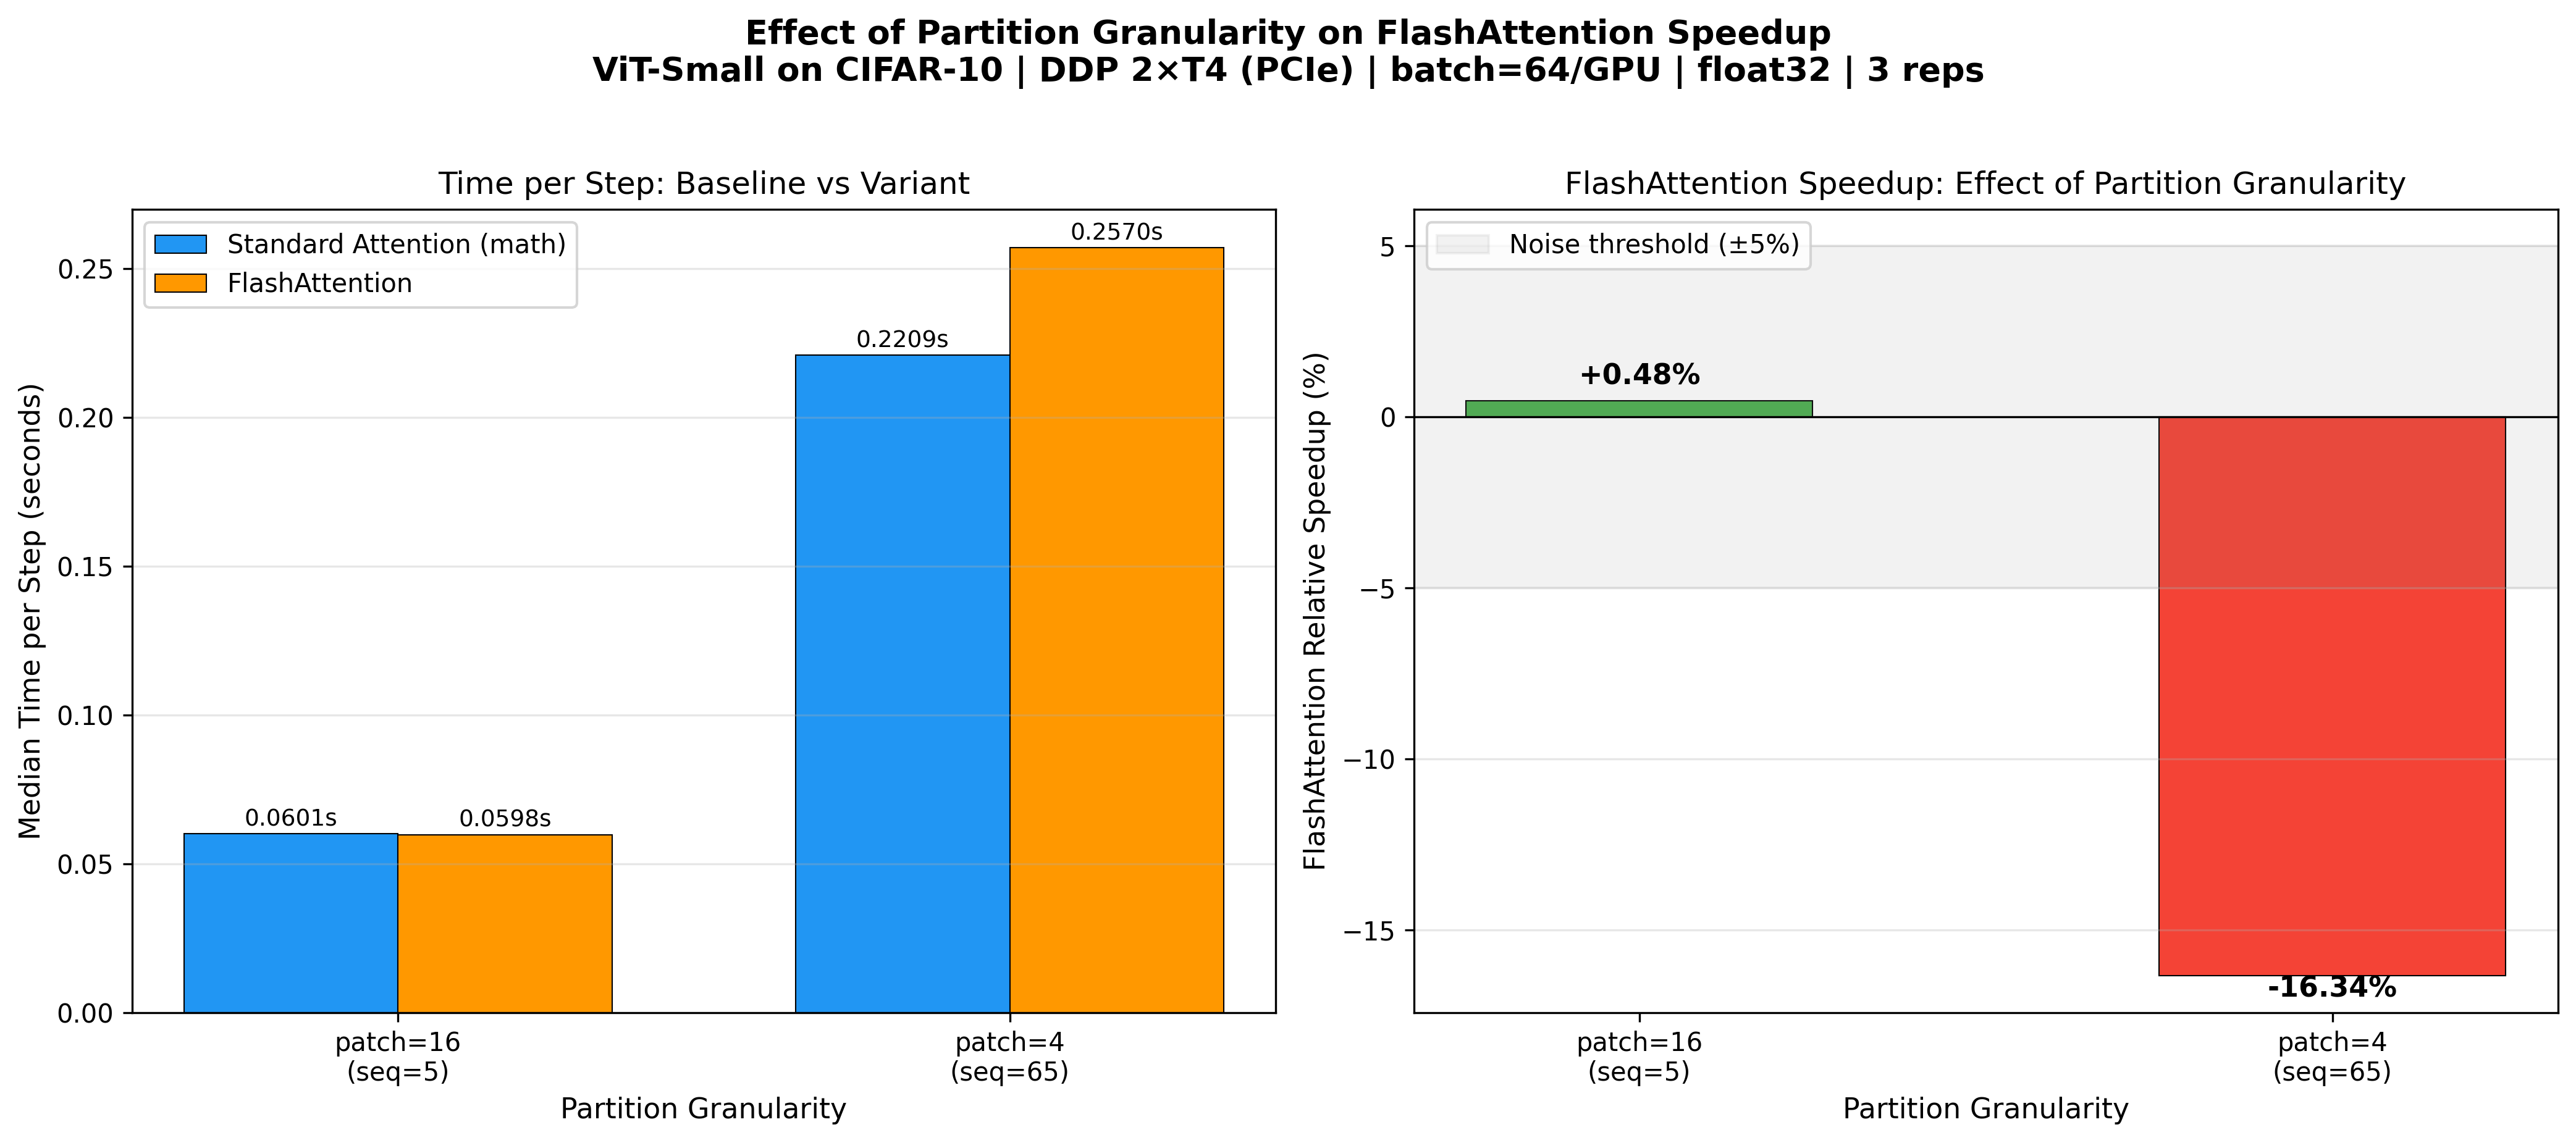
\includegraphics[width=0.75\textwidth]{../results/primary_figure.png}
\caption{A04 primary figure: median wall-clock time per training step at sequence lengths 5 and 65 tokens for math and \enquote{flash} kernels on two Tesla T4 GPUs. Source: \texttt{results/primary\_figure.png}.}
\label{fig:primary}
\end{figure}

\noindent The numerical summary of the primary figure is reproduced in Table~\ref{tab:a04-summary}.

\begin{table}[h!]
\centering
\caption{A04 primary result summary}
\label{tab:a04-summary}
\small
\begin{tabularx}{\textwidth}{l r r X r r}
\toprule
\textbf{Run} & \textbf{Patch size} & \textbf{Seq.\ length} & \textbf{Kernel requested} & \textbf{Median time/step (s)} & \textbf{Throughput (samples/s)} \\
\midrule
R1-baseline-std   & 16 &  5 & math  & 0.0601 & 2131.3 \\
R1-baseline-flash & 16 &  5 & flash & 0.0598 & 2141.5 \\
R2-variant-std    &  4 & 65 & math  & 0.2209 &  579.5 \\
R2-variant-flash  &  4 & 65 & flash & 0.2570 &  498.1 \\
\bottomrule
\end{tabularx}
\end{table}

\section{Interpretation of the Strong Result}

At the smaller sequence length (5 tokens, R1), the difference between \texttt{math} and \texttt{flash} requests is 0.5 percent, well inside the inter-replicate noise of the harness (replicate standard deviation approximately 1 to 1.5 milliseconds). At the larger sequence length (65 tokens, R2), the requested \texttt{flash} kernel is 16.3 percent slower than \texttt{math}. Three explanations are plausible. First, FlashAttention v1 may have an overhead that exceeds its IO benefit at 65 tokens on a Tesla T4; the literature places the FlashAttention crossover at higher sequence lengths on the A100, and the Tesla T4's HBM-to-SRAM bandwidth ratio could shift this crossover further to the right. Second, the PyTorch SDPA dispatcher may have silently fallen back to the memory-efficient kernel or the math kernel because Streaming Multiprocessor capability 7.5 (Turing) is below the 8.0 minimum for the FlashAttention SDPA backend~\parencite{pytorch2024sdpa}, in which case the comparison at 65 tokens is between two implementations of the math or memory-efficient algorithm with different harness overhead, not between FlashAttention and standard attention. Third, the Tesla T4 thermal envelope may have varied between R1 and R2; this is mitigated but not eliminated by the warmup and replication protocol. The author has reasonable confidence that the second explanation is the most likely, but treats it as an open question. Resolving this ambiguity is the first deliverable of ARE-II Sprint~1.

\section{Protocol Compliance Note}

The pilot was conducted on Kaggle's free-tier two-Tesla-T4 platform under FP32 precision, with the harness recording forward and backward time decomposition through CUDA events. Two protocol deviations from the originally pre-registered plan in A01 should be noted. First, the workload is a Vision Transformer on CIFAR-10 rather than a Large Language Model on LongBench; this deviation is driven by the hardware-fitness analysis in Part~III (a 7B-class Large Language Model does not fit in the 16-gigabyte HBM of the Tesla T4 even at FP16). Second, energy-per-token measurement was not performed in the pilot because the NVIDIA Management Library energy telemetry was not made reliably available through the Kaggle environment. Energy is therefore proposed as a Sprint~3 stretch metric pending a confirmed measurement path. Both deviations are made explicit here so that the committee can evaluate the protocol compliance of subsequent ARE-II evidence against the corrected baseline rather than against the original A01 thresholds.

\newpage

%==============================================================================
\part*{Part V --- Reproducibility}
\addcontentsline{toc}{part}{Part V --- Reproducibility}
%==============================================================================

\section{Reproduction Instructions}

The reproducible repository is co-located with this document. The repository structure is:

\begin{small}
\begin{verbatim}
.
|-- README.md                      # how to reproduce
|-- requirements.txt               # Python dependencies
|-- proposal/
|   |-- AREII_Ready_Package.tex    # this document
|   |-- references.bib
|-- related_work/                  # literature map, gap matrix, annotated bib
|-- configs/
|   |-- baseline.yaml              # A03 baseline (R1)
|   |-- variant.yaml               # A04 variant (R2)
|   |-- are_ii/
|       |-- sprint1_kernel_attribution.yaml
|       |-- sprint2_microbenchmark.yaml
|       |-- sprint3_full_model.yaml
|       |-- sprint4_a100_stretch.yaml
|-- src/
|   |-- dist_train.py              # cleaned distributed-training harness
|-- results/
    |-- primary_figure.png         # A04 primary figure
    |-- supporting_breakdown.png   # A04 forward/backward breakdown
    |-- summary.csv                # A04 summary table
    |-- all_results.json           # A04 full per-replicate data
\end{verbatim}
\end{small}

\noindent To reproduce the A04 strong result on a Kaggle notebook (two Tesla T4 GPUs):

\begin{enumerate}[leftmargin=2em]
    \item Create a new Kaggle notebook. Under \textit{Settings}, set the accelerator to \textit{GPU T4 x2}.
    \item Add the \texttt{cifar-10-python} dataset as a Kaggle input.
    \item Install the dependencies declared in \texttt{requirements.txt}.
    \item Run the harness once per (patch size, kernel) cell with: \texttt{torchrun --nproc\_per\_node=2 src/dist\_train.py PATCH\_SIZE USE\_FLASH OUTPUT.json}, with patch sizes 16 and 4 and \texttt{USE\_FLASH} in $\{0, 1\}$.
    \item Aggregate the four output JSON files into \texttt{results/summary.csv} and re-render \texttt{results/primary\_figure.png}.
\end{enumerate}

\noindent The full reproduction recipe, including environment setup commands, is in \texttt{README.md} at the repository root. The plot and table generation code is self-contained.

%==============================================================================
\newpage
\appendix

\section{AI Usage Log}
\label{app:ai-usage}

The following AI tools were used in the preparation of this package. Each entry records the tool, the purpose of use, the verification I performed, and the original intellectual contribution.

\begin{small}
\renewcommand{\arraystretch}{1.4}
\begin{tabularx}{\textwidth}{p{2.4cm} X p{3.0cm} p{3.4cm}}
\toprule
\textbf{Tool} & \textbf{Purpose} & \textbf{Independent verification} & \textbf{Original work} \\
\midrule
Claude Code (Anthropic) & Scaffolded the LaTeX bundle structure; assembled the literature map, gap matrix, annotated bibliography, and ARE-II execution plan from my A01--A04 materials; cross-checked GPU support claims for the Tesla T4 against PyTorch documentation, Dao-AILab GitHub issues, and the xFormers documentation via web search. & All technical claims (Streaming Multiprocessor capability of the Tesla T4, FlashAttention SDPA backend requirements, Tesla T4 unsupported status, xFormers Tesla T4 support, the existence of the Long-Context Attention Benchmark 2025 paper) verified against primary sources cited in the bibliography. & Research question, gap framing, hypotheses, ARE-II sprint structure, hardware path decisions, IP-safety filtering, the cautious-tone re-interpretation of A04, and the writing of every paragraph in this document are entirely my own. \\
\addlinespace
ChatGPT with Internet & Used during A01 and A02 for paper search and topic exploration; not used for new content in A05. & Cross-referenced against Google Scholar and arXiv. & A01 and A02 framing decisions are mine. \\
\addlinespace
NotebookLM (Gemini) & Used during A02 to summarize FlashAttention v1/v2/v3, BigBird, Longformer, Linformer, Performer, and Long Range Arena. & Summaries verified against the original PDFs. & Critical analysis and gap identification are mine. \\
\addlinespace
Elicit & Used during A02 to expand the literature net (KV-cache management, MQA/GQA, PagedAttention). & Returned papers verified for relevance and citation accuracy. & Selection criteria and synthesis are mine. \\
\addlinespace
Grammarly & Grammar, spelling, and style checks. & All accepted suggestions reviewed individually. & Final phrasing and technical claims are my responsibility. \\
\bottomrule
\end{tabularx}
\end{small}

\noindent\textbf{Disclaimer.} I remain responsible for the correctness, originality, and scholarly integrity of this submission.

%==============================================================================
\newpage
\nocite{*}
\printbibliography[title={References}]

\end{document}
